\documentclass[preview]{standalone}

\usepackage{amsmath}
\usepackage{amssymb}
\usepackage{stellar}
\usepackage{bettelini}
\usepackage{wrapfig}

\hypersetup{
    colorlinks=true,
    linkcolor=black,
    urlcolor=blue,
    pdftitle={Biologia},
    pdfpagemode=FullScreen,
}

\begin{document}

\title{Biologia}
\id{biologia-osmosi}
\genpage

\section{Osmosi}

\begin{snippet}{osmosi-expl}
    Le particelle nel soluto si spostano fra le membrane semi-permeabili secondo il gradiente
di concentrazione. Quando non è possibile raggiungere un equilibrio spostando il soluto,
l'equilibrio si può raggiunto per spostamento del solvente (acqua) piuttosto che il soluto.
\end{snippet}

\begin{snippetdefinition}{osmosi-definition}{Osmosi}
    Per \textit{osmosi} si intede il passaggio spontaneo dell'acqua (solvente) attraverso una membrana semi-permeabile
    per raggiungere un equilibrio elettrochimico.
\end{snippetdefinition}

\begin{snippetdefinition}{osmoregolazione-definition}{Osmoregolazione}
    Per \textit{osmoregolazione} si intende l'intervento attivo che fa l'organismo per evitare di subire le conseguenze del movimento spontaneo dell'acqua.
\end{snippetdefinition}

\begin{snippet}{equilibrio-idrico-illustration}
    \setlength{\intextsep}{0pt}%
    \begin{wrapfigure}{l}{0.60\textwidth}
        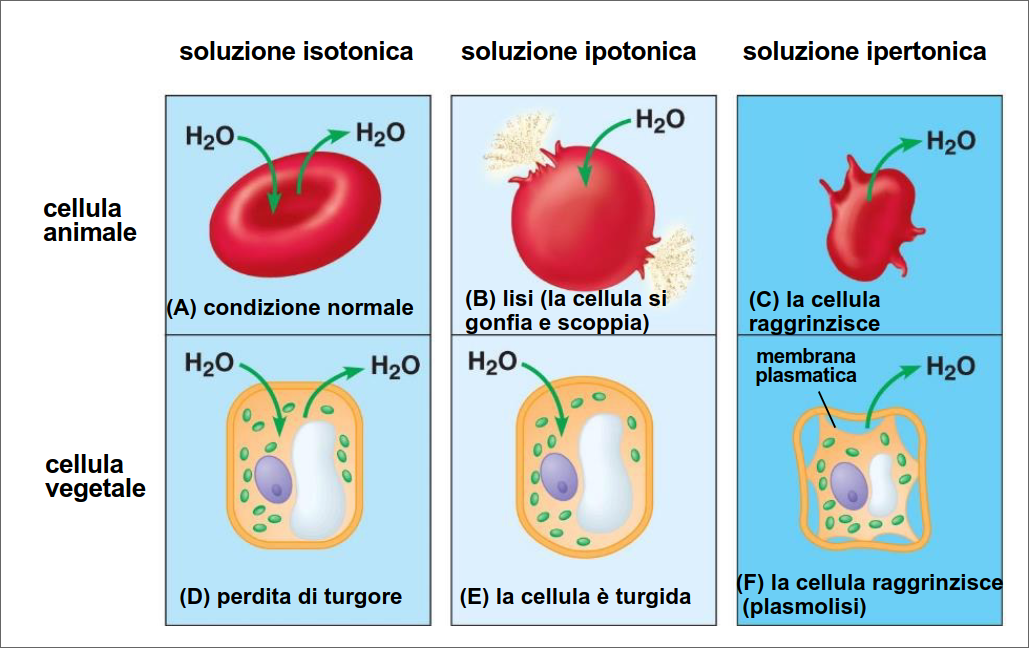
\includegraphics[width=0.6\textwidth]{./resources/equilibrio_idrico.png}
        \caption{Equilibrio idrico}
        \vspace{-1cm}
    \end{wrapfigure}

    Attraverso l'osmoregolazione è mantenuto costante il bilancio tra acqua e soluti
    nei fluidi corporei.

    Attraverso l'escrezione vengono rimossi i prodotti di scarto
    derivati dal catabolismo cellulare quindi organismi acquatici e terrestri sono in
    maggioranza osmoconformisti.

    La cellula vegetale non scoppia perché ha la parete per contenere.

    \wrapfill
\end{snippet}

\begin{snippetdefinition}{soluzione-isotonica-definition}{Soluzione isotonica}
    Una \textit{soluzione isotonico} è una soluzione che contiene la stessa
    concentrazione di acqua e soluti.
\end{snippetdefinition}

\begin{snippet}{soluzione-isotonica-expl}
    Se le concentrazioni di soluti sono
    uguali tra l'interno della cellula e l'ambiente circostante, non ci sarà
    alcun aumento o perdita netta di acqua dalla cellula. \\
    Nella cellula animale significa che la cellula si trova ad
    una condizione normale, sarà presente la stessa concentrazione di soluto
    da entrambe le parti e dunque si creerà un equilibrio idrico. Nella cellula
    vegetale invece una soluzione isotonica porta ad una perdita di turgore.
\end{snippet}

\begin{snippetdefinition}{soluzione-ipotonica-definition}{Soluzione ipotonica}
    Una \textit{soluzione ipotonica} è una soluzione una minore concentrazione di soluto rispetto ad
    altra soluzione.
\end{snippetdefinition}

\begin{snippet}{soluzione-ipotonica-expl}
    Se la soluzione è ipotonica rispetto alla cellula, l'acqua tenderà a scorrere verso
    l'interno di essa e la cellula reagirà prima gonfiandosi e poi scoppiando: dando luogo alla cosiddetta lisi
    cellulare. Nella cellula vegetale la soluzione ipotonica porta la cellula ad una condizione favorevole e
    ideale, la cellula è turgida perché ha bisogno di più acqua, non scoppierà perché ha la parete.
\end{snippet}

\begin{snippetdefinition}{soluzione-ipertonica-definition}{Soluzione ipertonica}
    sono caratterizzate da una maggiore concentrazione di soluto rispetto a
    qualsiasi altra soluzione.
\end{snippetdefinition}

\begin{snippet}{soluzione-ipertonica-expl}
    Quando la soluzione è tale, rispetto a una cellula l'acqua tenderà ad andare
    verso l'esterno della stessa che, quindi, rischierà di danneggiarsi a causa della disidratazione. La cellula
    vegetale si raggrinzisce perché l'acqua esce da essa, questa situazione si chiama plasmolisi.
\end{snippet}

\end{document}